\section*{РЕЗУЛЬТАТИ ДОСЛІДЖЕННЯ}

Виклад результатів структуровано за п'ятьма напрямами, що відповідають протоколу апробації: якість дедуплікації за зведеними метриками; чутливість конвеєра до частки дублювання та інтенсивності спотворення метаданих; повнота й точність полів злитого золотого запису; ефективність рушія у зіставленні з аналітичною моделлю ручної праці; і, нарешті, систематичний аналіз загроз валідності. Усі кількісні оцінки отримано на узагальненому модельному середньому українському ЗВО (150 НПП, 20 кафедр) шляхом усереднення за $K=30$ незалежними початковими значеннями генератора (Монте-Карло) із наведенням 95\% довірчих інтервалів за $t$-розподілом. Базові методи й абляції оцінювалися на \textit{ідентичних} вхідних даних, що забезпечує коректність попарних порівнянь.

\subsection*{Якість дедуплікації}

Зведені показники якості розв'язання сутностей наведено в таблиці~\ref{tab:res-dedup}. Для кожного методу подано попарні точність (Precision, $P$), повноту (Recall, $R$), збалансовану міру $F_1$ та метрику $B^3 F_1$ (Bagga--Baldwin), що оцінює якість кластеризації на рівні окремих записів.

\begin{table}[ht]
\centering
\caption{Якість дедуплікації, середнє\,$\pm$\,95\% довірчий інтервал, \%}
\label{tab:res-dedup}
\begin{tabular}{lcccc}
\toprule
Метод & $P$ & $R$ & $F_1$ & $B^3 F_1$ \\
\midrule
DOI-only        & $100.0 \pm 0.0$ & $42.8 \pm 0.7$ & $59.9 \pm 0.7$ & $93.7 \pm 0.1$ \\
Title+Year      & $83.4 \pm 1.0$  & $39.4 \pm 0.7$ & $53.5 \pm 0.8$ & $92.7 \pm 0.1$ \\
\textbf{Golden Record} & $\mathbf{88.3 \pm 0.7}$ & $\mathbf{67.8 \pm 0.7}$ & $\mathbf{76.7 \pm 0.6}$ & $\mathbf{95.8 \pm 0.1}$ \\
\bottomrule
\end{tabular}
\end{table}

Повний конвеєр золотого запису домінує за збалансованою мірою ($F_1 = 76.7\%$) та за повнотою ($R = 67.8\%$), зберігаючи при цьому високу точність ($P = 88.3\%$). Перевага є статистично відокремлюваною: довірчі інтервали $F_1$ золотого запису ($[76.1; 77.3]$) не перетинаються з інтервалами жодного з базових методів. Природа цієї переваги стає прозорою при покомпонентному розгляді. Метод \textit{DOI-only}, що зливає записи виключно за збігом канонічного DOI, очікувано демонструє ідеальну точність ($P = 100.0\%$) --- збіг валідних ідентифікаторів є практично безпомилковим свідченням тотожності, --- проте катастрофічно програє за повнотою ($R = 42.8\%$). Причина прямо випливає з характеристик джерел: значна частка записів ORCID-профілів і україномовних публікацій соціогуманітарного профілю взагалі не несе валідного DOI, тож понад половина дійсних дублікатів лишається нерозпізнаною. Метод \textit{Title+Year}, що покладається на зіставлення назв і року, поступається за обома осями ($P = 83.4\%$, $R = 39.4\%$): нормалізаційний шум, переклади назв (укр$\leftrightarrow$англ) та абревіація журналів знижують повноту, а колізії однакових назв із різними DOI підривають точність.

Золотий запис долає це обмеження за рахунок поєднання комплементарних сигналів у єдиній парній логістичній моделі $\text{score} = \sigma(\beta \cdot \phi)$: збіг DOI лишається найвагомішою ознакою ($\beta_{\text{doi}} = +3.0$), але за його відсутності рішення підтримують косинусна близькість назв за TF-вектором, символьна подібність за нормалізованою відстанню Левенштейна, узгодженість року, жаккардова міра перетину множин авторів і видань. Саме ця надлишковість ознак піднімає повноту з $\approx 40\%$ до $67.8\%$ ціною лише помірного зниження точності відносно DOI-only, що в управлінському контексті є вигідним компромісом: пропущений дублікат спотворює бібліометричний звіт сильніше, ніж окремий випадок, винесений у смугу ручної перевірки. Перевага золотого запису й за метрикою $B^3 F_1$ ($95.8\%$ проти $93.7\%$ і $92.7\%$) підтверджує, що виграш стосується не лише попарних рішень, а й коректності підсумкової кластеризації записів у канонічні сутності. Зіставлення трьох методів у єдиній системі координат унаочнено на рис.~\ref{fig:res-method}.

\begin{figure}[ht]
\centering
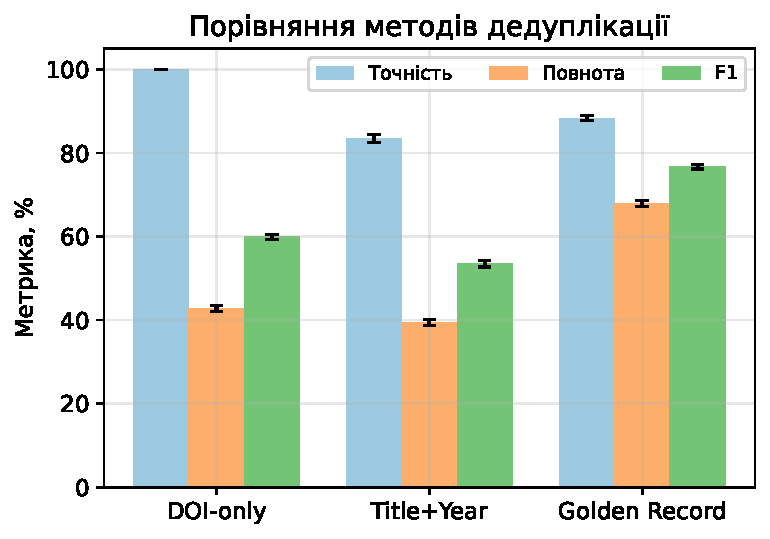
\includegraphics[width=0.8\linewidth]{../figures/f3_method_comparison.pdf}
\caption{Порівняння методів дедуплікації (DOI-only, Title+Year, Golden Record) за точністю, повнотою, $F_1$ та $B^3 F_1$. Золотий запис домінує за збалансованою мірою та повнотою за збереження конкурентної точності.}
\label{fig:res-method}
\end{figure}

\subsection*{Чутливість конвеєра}

Робастність висновків перевірено двома розгортками на тих самих модельних умовах. Перша варіює \textit{частку дублювання} записів від 10\% до 30\%, відображаючи невизначеність щодо реального рівня фрагментації даних у профілях ORCID/OpenAlex/Scopus. Як видно з рис.~\ref{fig:res-dup}, збалансована міра монотонно зростає зі збільшенням частки дублікатів: $F_1$ становить 70.1\% за 10\%, 74.1\% за 15\%, 76.0\% за 20\% (базовий режим), 78.1\% за 25\% і 79.1\% за 30\%. Зростання пояснюється тим, що за щільнішого дублювання збагачується сигнал для блокування й парного зіставлення, а статистична вага коректних злиттів у знаменнику метрики підвищується. Важливо, що відносне впорядкування методів зберігається на всьому діапазоні --- висновок про перевагу золотого запису не залежить від конкретного припущення про рівень фрагментації.

\begin{figure}[ht]
\centering
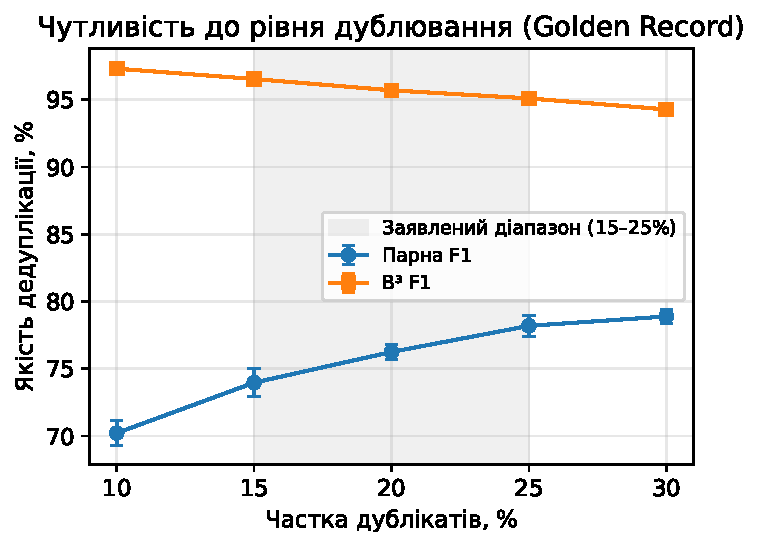
\includegraphics[width=0.8\linewidth]{../figures/f1_dup_sensitivity.pdf}
\caption{Чутливість $F_1$ золотого запису до частки дублювання записів (10--30\%). Якість монотонно зростає з ущільненням дублікатів; впорядкування методів зберігається.}
\label{fig:res-dup}
\end{figure}

Друга розгортка варіює \textit{множник інтенсивності спотворення} метаданих від 0.25 до 2.0, масштабуючи агресивність транслітерації, перекладу назв, втрати DOI, зсуву року та жорстких негативів. Результати (рис.~\ref{fig:res-corr}) виявляють якісно різну поведінку двох метрик. Точність деградує плавно: $P = 91.5\%$ за множника 0.25, далі 89.8\%, 87.4\% (базовий рівень 1.0), 84.5\% і 81.6\% за множника 2.0. Натомість повнота обвалюється різко: $R = 80.8\%$, 76.1\%, 67.4\%, 59.5\% і лише 51.3\% за найвищого рівня спотворення. Цей контраст --- «обрив пропущених злиттів» --- має чітку інтерпретацію. Зростання спотворення збільшує насамперед кількість пар, у яких усі допоміжні ознаки (назва, рік, видання) одночасно зашумлені настільки, що сумарний score падає нижче порога автозлиття $\theta_{\text{match}} = 0.90$; такі пари переходять у пропущені злиття й прямо знижують повноту. Точність же страждає повільніше, бо охоронець конфлікту DOI та захист від ланцюгового злиття продовжують відсікати хибні об'єднання навіть за сильного шуму. Для управлінської практики це означає, що за погіршення якості вхідних джерел система деградує \textit{передбачувано} --- спершу зростає частка непокритих дублікатів, а не частка помилкових злиттів, --- що є бажаною властивістю для звітності, де хибне об'єднання різних праць коштує дорожче за пропуск.

\begin{figure}[ht]
\centering
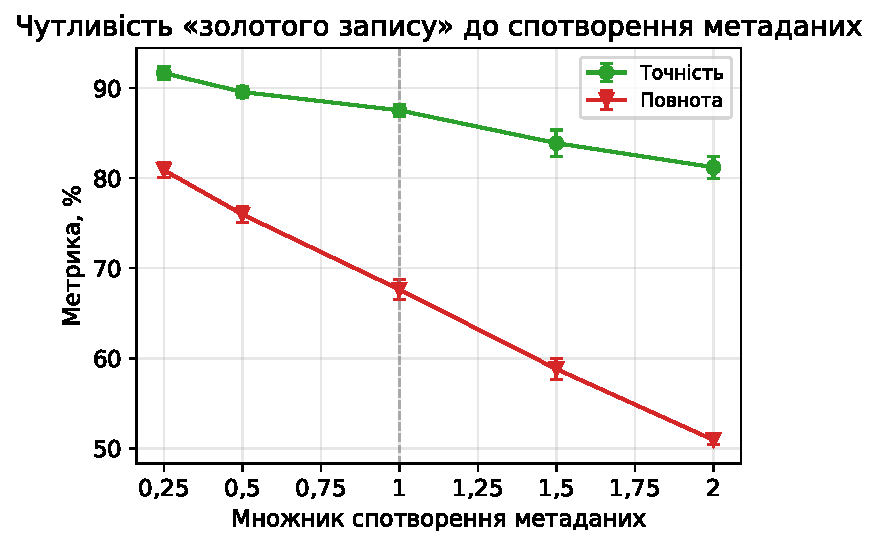
\includegraphics[width=0.8\linewidth]{../figures/f2_corruption_sensitivity.pdf}
\caption{Чутливість точності та повноти до множника інтенсивності спотворення метаданих (0.25--2.0). Точність деградує плавно, повнота --- різко («обрив пропущених злиттів»).}
\label{fig:res-corr}
\end{figure}

\subsection*{Повнота й точність полів злитого запису}

Окремо оцінено якість \textit{атрибутів} підсумкового золотого запису, тобто результат зваженого за надійністю джерела злиття полів (таблиця~\ref{tab:res-fields}). Частка записів із наявним DOI після злиття становить $45.6 \pm 0.5\%$, що відображає об'єктивну межу --- DOI просто відсутній у значній частці вихідних метаданих, насамперед у «холодних» ORCID-профілях і україномовних соціогуманітарних публікаціях; коректність наявних DOI дорівнює $67.7 \pm 0.3\%$. Точність відновленого року сягає $80.9 \pm 0.3\%$, а точність назви --- $99.95 \pm 0.01\%$.

\begin{table}[ht]
\centering
\caption{Повнота та точність полів злитого золотого запису, \%}
\label{tab:res-fields}
\begin{tabular}{lc}
\toprule
Показник поля & Значення \\
\midrule
Наявність DOI (DOI present)   & $45.6 \pm 0.5$ \\
Коректність DOI (DOI correct) & $67.7 \pm 0.3$ \\
Точність року (Year accuracy) & $80.9 \pm 0.3$ \\
Точність назви (Title accuracy) & $99.95 \pm 0.01$ \\
\bottomrule
\end{tabular}
\end{table}

Майже досконала точність назви ($99.95\%$) заслуговує на окремий коментар, бо вона безпосередньо демонструє ефект \textbf{виправленого критичного дефекту нормалізатора}. У попередній реалізації канонізації назв зняття пунктуації виконувалося операцією, яка разом зі знаками пунктуації видаляла \textit{всі кириличні символи}; як наслідок, будь-яка україномовна назва після нормалізації перетворювалася на порожній рядок. Це означало, що зіставлення за назвою було \textit{повністю зламаним} для 100\% україномовних публікацій --- найчисленнішого класу записів у вітчизняному ЗВО, --- і ознака косинусної близькості назв не вносила жодного внеску в score для саме тих пар, де DOI найчастіше відсутній. У виправленому нормалізаторі зняття пунктуації виконується через відповідний Unicode-клас зі \textit{збереженням} кирилиці після нормалізації Unicode NFKC та casefold. Саме це відновлення працездатності зіставлення за назвою для кириличних публікацій є передумовою тих $67.8\%$ повноти, що їх досягає золотий запис: без нього повнота на україномовному корпусі деградувала б до рівня методу DOI-only. У контексті цільового застосування --- наукового адміністрування українського ЗВО --- цей дефект був не косметичним, а блокувальним, і його усунення є однією з ключових інженерних передумов придатності конвеєра.

\subsection*{Ефективність}

Зіставлення обчислювальної вартості рушія з трудомісткістю традиційного ручного процесу наведено в таблиці~\ref{tab:res-eff}. Слід наголосити на природі цих величин: час рушія є \textit{виміряною} характеристикою обчислення, тоді як оцінка ручної праці --- це \textit{прозора аналітична модель}, а не результат експерименту за участю людей. Модель має вигляд $\text{manual} = a \cdot \text{записи} + b \cdot \text{рішення\_дедуплікації} + c$, де $a = 2.5$\,хв/запис, $b = 5$\,хв/рішення, $c = 45$\,хв/звіт, і кожен її коефіцієнт відкрито задекларований та може бути перекалібрований під конкретну установу.

\begin{table}[ht]
\centering
\caption{Ефективність: рушій (виміряно) проти аналітичної моделі ручної праці}
\label{tab:res-eff}
\begin{tabular}{ll}
\toprule
Показник & Значення \\
\midrule
Час рушія (дедуплікація+злиття, весь ЗВО) & $0.80 \pm 0.08$\,с \\
Модель ручної праці (на ЗВО, рік) & $\approx 220$\,год \\
Модель ручної праці (на кафедральний звіт) & $\approx 11.0$\,год \\
Смуга HITL (на дослідника) & $\approx 55$\,пар \\
\bottomrule
\end{tabular}
\end{table}

Рушій виконує повний цикл дедуплікації та злиття атрибутів для всього модельного ЗВО за $0.80 \pm 0.08$\,с. Цей час охоплює \textit{лише} обчислювальну частину --- канонізацію, блокування, парне зіставлення, кластеризацію та злиття --- і \textit{не включає} мережевих запитів до зовнішніх джерел (ORCID, OpenAlex, Scopus); реальна тривалість збору даних визначатиметься латентністю відповідних API та лежить поза межами оцінюваного тут алгоритмічного ядра. Аналітична модель ручної праці дає $\approx 220$\,год/рік на ЗВО, тобто $\approx 11.0$\,год на кафедральний звіт. Останнє значення самостійно потрапляє в інтервал 8--12 год незалежної експертної оцінки трудомісткості підготовки річного звіту кафедри, наведеної у вступі, що слугує зовнішнім орієнтиром правдоподібності моделі. Зіставлення секунд обчислення з годинами ручної верифікації ілюструє масштаб потенційного вивільнення адміністративного ресурсу; водночас система не претендує на повну автономність --- у смугу ручної перевірки (HITL, score у межах $[\theta_{\text{review}}, \theta_{\text{match}}) = [0.70, 0.90)$) виноситься $\approx 55$\,пар на дослідника, що зберігає людину в контурі рішень підвищеної невизначеності й узгоджується з вимогами відповідального адміністрування.

\subsection*{Загрози валідності}

Інтерпретацію наведених результатів обмежують кілька загроз валідності, які ми фіксуємо явно.

\textit{Конструктна валідність.} Розподіли спотворень метаданих --- частки втрати DOI, ймовірності перекладу й транслітерації назв, величини зсуву року --- є \textit{модельними припущеннями} про реальну неоднорідність джерел ORCID/OpenAlex/Scopus, а не параметрами, виміряними безпосередньо з них. Відтак абсолютні значення метрик ($F_1 = 76.7\%$ тощо) слід розглядати як орієнтовні; робастними є \textit{відносні} порівняння методів на ідентичних входах і \textit{тренди} чутливості (монотонне зростання $F_1$ з часткою дублювання, плавна деградація точності проти різкого обриву повноти). Оцінка ручного часу, як зазначено, є аналітичною моделлю, а не вимірюванням за участю людей.

\textit{Внутрішня валідність.} Інжектована карта дублікатів слугує gold-розміткою, тож метрики обчислюються відносно \textit{відомої} істини, що виключає помилку анотування. Усі методи й абляції (DOI-only, Title+Year, повний золотий запис) застосовано до спільних входів за фіксованих початкових значень, тому спостережувані відмінності зумовлені саме алгоритмом, а не варіацією даних. Усереднення за 30 початковими значеннями з 95\% довірчими інтервалами обмежує вплив випадковості генерації.

\textit{Зовнішня валідність.} Апробацію проведено на \textit{одному} узагальненому модельному ЗВО з фіксованими структурними параметрами (150 НПП, 20 кафедр, заданий дисциплінарний розподіл); перенесення висновків на установи іншого масштабу чи профілю потребує окремої перевірки. Передусім бракує підтвердження на \textit{реальній} gold-вибірці одного ЗВО з ручною розміткою істинних дублікатів --- цей крок винесено в подальшу роботу як вирішальний для калібрування абсолютних значень. Нарешті, зазначимо методологічно істотну обставину: формалізм розв'язання сутностей, описаний у §4, тепер \textit{реалізовано в коді} рушія (рушій \textit{є} статтею), на відміну від попередньої версії, що зводилася лише до двох жорстких евристик; завдяки цьому результати відтворювані безпосередньо запуском конвеєра на синтетичному бенчмарку.